\chapter{Theory}
In this chapter we explain the theoretical concepts relevant to this thesis. We start with explaining the physics behind our method in section \ref{bubble_physics}, in particular how bubbles interact with light. Next, we discuss the mathematical basics necessary for image processing such as Fourier theory and convolution in section \ref{image_processing}. Section \ref{machine_learning} explains the principle behind machine learning that our method relies on for classification. Finally, section \ref{the_object_detection_problem} formally introduces the object detection problem and our chosen criteria for evaluation. 

	\section{Bubble physics} \label{bubble_physics}
	
	\section{Image processing}	\label{image_processing}
	In the following we represent an image as a two dimensional signal written as a matrix \textit{\textbf{g}}. Therefore, $g_{m,n}$ denotes the pixel (i.e. picture element) at the \textit{m}-th row corresponding to the \textit{n}-th column. The chosen coordinate system is described in figure \ref{fig:coord_sys}. 
	
		\begin{figure}
		    \centering
		    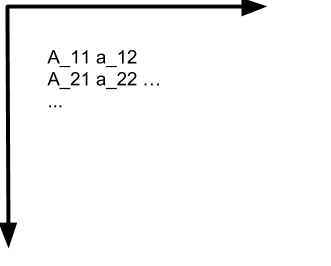
\includegraphics[scale=0.4]{images/coord_sys.png}
		    \caption{Notation and coordinate system}
		    \label{fig:coord_sys}
		\end{figure}
	
		\subsection{Fourier theory}
		The Fourier transform is an important image processing tool which is used to decompose an image into its since and cosine components. The output of the transformation represents the image in the Fourier or frequency domain, while the input image is the spacial domain. In the Fourier domain image, each point represents a particular frequency contained in the spatial domain image.
		The \textit{continuous} two-dimensional Fourier transform is defined as
		\begin{equation}
				\mathscr{F}\{ g(\mathbf{x})  \} = \hat{g}(\mathbf{k}) = 
				\int_{-\infty}^{\infty} g(\mathbf{x}) \text{exp}\left( -2 \pi \text{i} \mathbf{k}^T \mathbf{x}  \right) \text{d}\mathbf{x}
		\end{equation}
		and the inverse Fourier transform
		\begin{equation}
				\mathscr{F}^{-1}\{ \hat{g}(\mathbf{k}) \} = g(\mathbf{x}) =
				 \int_{-\infty}^{\infty} \hat{g}(\mathbf{k})
			\text{exp}\left( -2 \pi \text{i} \mathbf{k}^T \mathbf{x}  \right) \text{d}\mathbf{x}
		\end{equation}
		Where $\mathbf{x}$ and $\mathbf{k}$  are the two dimensional space and frequency vectors respectively. 
		
		Images however are discrete two dimensional signals, we therefore need to apply the \textit{Discrete} Fourier transform or DFT, defined as
		\begin{equation}
			\text{DFT}\{ g_{m,n} \} = \hat{g}_{u,v} = \dfrac{1}{MN} \sum_{m=0}^{M-1} \sum_{n=0}^{N-1}
			g_{m,n} \text{ exp} \left(  - \dfrac{2 \pi \text{i} m u}{M}  \right)
						\text{exp} \left(  - \dfrac{2 \pi \text{i} n u}{N}  \right)
		\end{equation}		 

		Similarly, the inverse 2-D DFT is defined as 
		
		\begin{equation}
		 \text{IDFT}\{\hat{g}_{u,v}\} = g_{m,n} = \sum_{m=0}^{M-1} \sum_{n=0}^{N-1} \hat{g}_{u,v}
			\text{ exp} \left(   \dfrac{2 \pi \text{i} m u}{M}  \right)
			\text{exp} \left(   \dfrac{2 \pi \text{i} n u}{N}  \right)
		\end{equation}
		
		
		\subsection{Convolution}
		Convolution is one of the most important operations in signal processing. Convolving two signals $g$ and $h$ produces a third signal that expresses how the shape of one is modified by the other. Formally, we define the continuous convolution as follows
		\begin{equation}
			(g \star h)(\mathbf{x}) = \int_{-\infty}^{\infty} 
			h(\mathbf{x}') g(\mathbf{x} - \mathbf{x}')
			\text{d}\mathbf{x}
		\end{equation}
		and the discrete two dimensional convolution as
		\begin{equation}
			g'_{m,n} = \sum_{m'=0}^{M-1} \sum_{n'=0}^{N-1}
			h_{m',n'} g_{m-m', n-n'}
		\end{equation}
		
		One important property of convolution is that we can express it as a multiplication in the Fourier domain. 
		\begin{equation}
		\mathscr{F}\{g \star h\} = N M \hat{h} \hat{g}
		\end{equation}
		This property, together with the fast Fourier implementation of the Fourier transform allows a fast computation of convolutions. 
		
		At the edge of the image, we typically extend the image with zero values (i.e. zero padding). This introduces an error when applying filters at the image border and we will mostly exclude the border when using filters (see chapter \ref{the_algorithm} for more details).
		
		\subsection{Smoothing}\label{sect:smoothing}
		Smoothing an image means convolving an image with a smoothing filter. A smoothing or averaging filters must ideally fulfill following conditions
		\begin{enumerate}
			\item Zero-shift: $\Im (\hat{h}(\mathbf{k})) = 0$
			\item Preservation of mean value: $\hat{h}(0) = 1 $
			\item Monotonous decrease: $ \hat{h}(k_1) \leq \hat{h}(k_2) $ for $ k_2 > k_2 $
			\item Isotropy: $\hat{h}(\mathbf{k}) = \hat{h}(| \mathbf{k} |)$ \textcolor{red}{stimmt das ??}
		\end{enumerate}
		
		In this work, we will be using Gaussian filters for one and two dimensional smoothing. Although Gaussian filters are not ideal, e.g. isotropy is violated for small standard deviations, it is still a good approximation for an ideal low pass filter. Computing the Fourier transform (for convolution) is also faster for a Gaussian filter. The $m$-th component of a one dimensional Gaussian filter mask can be obtained from the Gaussian function
		\begin{equation}
		G_{m} = \dfrac{1}{2 \pi \sigma^2} \text{ exp}
			 \left( 
			 	- \dfrac{(m-\mu)^2}{2 \sigma^2}
			 \right)
		\end{equation}
		Where $\mu$ is the mean, i.e. Gaussian peak's position and $\sigma$ is the standard deviation, i.e. peak's width.
		
		Figure \ref{fig:gauss_intro} show a Gaussian curve in one and two dimensions as well as the result of convolving an image with a Gaussian filter mask. Note how the image becomes blurry, i.e. large wave numbers have been suppressed.
		\begin{figure}
		    \centering
		    \begin{subfigure}[b]{0.3\textwidth}
		        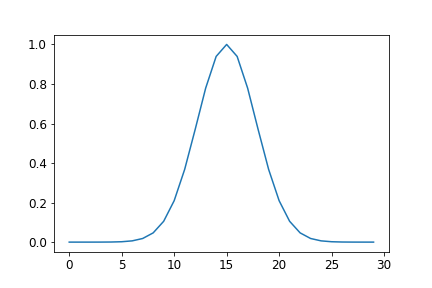
\includegraphics[width=\textwidth]{graphs/gauss_sigma_2.png}
		        \caption{1D Gaussian signal with $\mu=15$ and $\sigma=2$}
		    \end{subfigure}
		    
		    \begin{subfigure}[b]{0.3\textwidth}
		        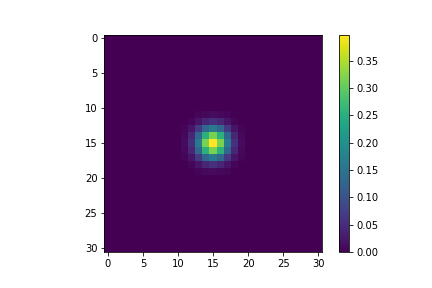
\includegraphics[width=\textwidth]{images/gauss_sigma_2.png}
		        \caption{2D Gaussian signal with $\mu_x = \mu_y = 15$ and $\sigma_x = \sigma_y = 2$}
		    \end{subfigure}
		    
		    \begin{subfigure}[b]{0.3\textwidth}
		        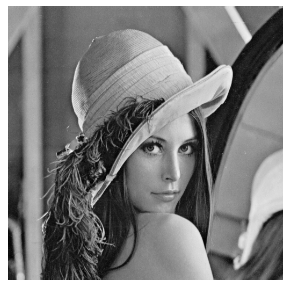
\includegraphics[width=\textwidth]{images/lena_orig.png}
		        \caption{Original image}
		    \end{subfigure}
		    ~ %add desired spacing between images, e. g. ~, \quad, \qquad, \hfill etc. 
		      %(or a blank line to force the subfigure onto a new line)
		    \begin{subfigure}[b]{0.3\textwidth}
		        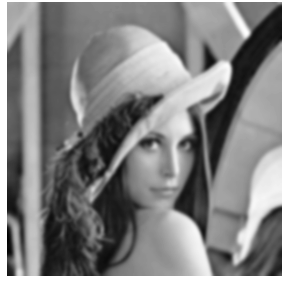
\includegraphics[width=\textwidth]{images/lena_smooth.png}
		        \caption{After convolution with 2D Gaussian mask}
		    \end{subfigure}
		    ~ %add desired spacing between images, e. g. ~, \quad, \qquad, \hfill etc. 
		    %(or a blank line to force the subfigure onto a new line)

		    \caption{Gaussian smoothing filter}
		    \label{fig:gauss_intro}
		\end{figure}




		\subsection{Edges and Derivation}
		\begin{figure}\label{fig:edges_intro}
			\centering
			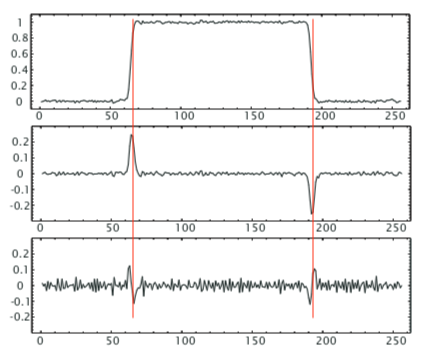
\includegraphics[scale=0.8]{graphs/edges_intro.png}
			\caption{Original 1D signal. First derivative. Second derivative}
		\end{figure}
		An edge can be defined as a set of continuous pixel positions where an abrupt change of intensity (i.e. gray value) occurs. Therefore, edge detection is based on differentiation, where in discrete images differentiation is replaced by discrete differences that are mere approximation to differentiation. There is also the need to not only know where edges are, but also how strong they are. Figure \ref{fig:edges_intro} shows that in the one dimensional case, edges can be detected by applying first and second derivatives to the signal. 
		
		In continuous space, a partial derivative operation is defined as
		\begin{equation}
		 	\mathbf{\nabla} = \left[ \dfrac{\partial}{\partial x}, \dfrac{\partial}{\partial y} \right]
		\end{equation}
		and its corresponding Fourier transform is
		\begin{equation}
			\mathscr{F}\{\mathbf{\nabla}\} = 2 \pi \text{i} \mathbf{k}
		\end{equation}
		
		For the second derivative we need to consider all possible combinations of second order partial differential operators of a two dimensional signal. The resulting $2 \times 2$ matrix is called the Hessian matrix
		\begin{equation}
			\mathbf{H} = 
				\begin{bmatrix}
   \dfrac{\partial^2}{\partial x^2}       & \dfrac{\partial^2}{\partial x \partial y}\\
   \dfrac{\partial^2}{\partial y \partial x}       & \dfrac{\partial^2}{\partial y^2}\\
				\end{bmatrix}
		\end{equation}
		and its Fourier transform is
		
		\begin{equation}
			\mathscr{F}\{\mathbf{H}\} = -4 \pi^2 \mathbf{k}\mathbf{k}^T
		\end{equation}
		
		
		Edge detectors can be implemented as filters $h$ that operate on a two dimensional grid. From the above equations we can derive the general properties for these filters:
		\begin{enumerate}
			\item Zero-shift: 
				\begin{itemize}
					\item $90^\circ$ phase shift for first order derivative, implying $ \Im\{ \hat{h} \} \neq 0$ and an antisymmetric filter mask, i.e $h_{-n} = -h_{n}$
					\item a second order derivative operator must be symmetric in order to satisfy the zero shift property, i.e. $h_{-n} = h_{n}$
				\end{itemize} 
				
			\item Suppression of mean value: $\hat{h}(k_i =0) \Leftrightarrow \sum_{\mathbf{n}}h_{\mathbf{n}} = 0$
			
			\item isotropy: For good edge detection, the edge detector's response must not depend on the direction of the edge. 
				\begin{itemize}
					\item first order derivative $\hat{h}(\mathbf{k}) = 
											\pi \text{i} k_i \hat{b} (|\mathbf{k}|)$
					\item second order derivative $\hat{h}(\mathbf{k}) = 
											\pi^2 k_i^2 \hat{b} (|\mathbf{k}|)$
				\end{itemize}
				where $k_i$ denotes the wave number in the $i$-th direction and $b$ is an isotropic smoothing filter that fulfills the conditions
				\begin{equation}
					\hat{b}(\mathbf{0}) = 1, \hspace{1cm} \mathbf{\nabla}_k \hat{b}(|\mathbf{k}|) = \mathbf{0}
				\end{equation}
		\end{enumerate}
			
		In this work we will be using the Sobel filter masks as defined in equation (\ref{eq:sobel}) in order to compute derivatives in $x$ and $y$ directions. 
		\begin{equation}
			S_x =
			 \begin{bmatrix}
     				1	& 2 & 1 \\
    					0	 & 0 & 0 \\
    					-1	 & -2 & -1 \\
				\end{bmatrix},
			\hspace{2cm}
			S_y = 
				\begin{bmatrix}
     				1	& 0 & -1 \\
    					2	 & 0 & 2 \\
    					1	 & 0 & -1 \\
				\end{bmatrix}
			\label{eq:sobel}
			\end{equation}
		At each point in the image, the resulting gradient approximations can be combined to give the gradient magnitude image $S$ using:
		\begin{equation}
			S = \sqrt{(S_x \star G )^2 + (S_y \star G)^2}
			\label{eq:grad_sobel}
		\end{equation}

%		as well as the orientation $\theta$
%		\begin{equation}
%			\theta = \arctan \left(\dfrac{S_y \star G}{S_x \star G}\right)
%		\end{equation}

		where G is the input image. Figure \ref{fig:sobel_demo} shows the result of applying the derivation operator on an image. Note how edges have different magnitude depending on their strength. 

		\begin{figure}
			\centering
			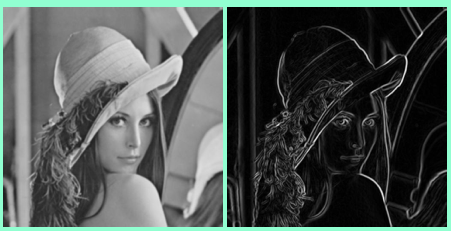
\includegraphics[scale=0.5]{images/lena_orig_sobel.png}
			\caption{Left: original image. Right: gradient image}
			\label{fig:sobel_demo}
		\end{figure}
		
		
		\subsection{Orientation and Structure Tensor}
		\begin{figure} %fig:struct_tensor_intro
			\centering
			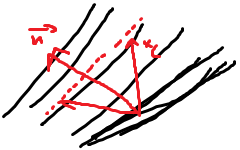
\includegraphics[scale=1]{images/structure_tensor_intro.png}
			\caption{Ideal local neighborhood described by a unit vector $\tilde{\mathbf{n}}$}
			\label{fig:struct_tensor_intro}
		\end{figure}
		Although derivation is useful to determine the gradient magnitude and its direction in an image, it doesn't tell us much about gradient directions in a specific neighborhood of a point. Figure \ref{fig:struct_tensor_intro} shows that in a neighborhood with ideal orientation gray values change in one direction only. Generally, the direction of local orientation can be denoted with a unit vector $\tilde{\mathbf{n}}$. If we orient the coordinate system along the principal directions, the gray values become a one dimensional function and a simple neighbourhood can be represented by
		\begin{equation}
			g(\mathbf{x}) = g(\mathbf{x}^T \tilde{\mathbf{n}})
		\end{equation}

		The drawback of this representation however, is that it cannot distinguish between neighborhoods with constant values and isotropic orientation distribution. So if we define the optimum orientation as the orientation that shows the least deviations from the directions of the gradient, we can expressed it using the unit vector $\tilde{\mathbf{n}}$ as
		\begin{equation}
			\mathbf{\nabla}g^T \tilde{\mathbf{n}} = \cos[\angle(\mathbf{\nabla}g, \tilde{\mathbf{n}})]\\
			\Leftrightarrow \\
			\left( \mathbf{\nabla}g^T \tilde{\mathbf{n}} \right)^2 = 
						 |\mathbf{\nabla}g|^2 \cos^2[\angle(\mathbf{\nabla}g, \tilde{\mathbf{n}})]
		\end{equation}
		We can see that this quantity is maximized when the orientation is along the unit vector $\tilde{\mathbf{n}}$, i.e. when $\mathbf{\nabla}g$ and $\tilde{\mathbf{n}}$ are either parallel or antiparallel. Therefore, the following integral is maximized in a local neighborhood:
		\begin{equation}
			\int w(\mathbf{x} - \mathbf{x'}) 
								\left( 
									 \mathbf{\nabla}g(\mathbf{x'})^T \tilde{\mathbf{n}}
								\right)^2
								\text{d}\mathbf{x'}
			\label{eq:max_integral}
		\end{equation}
		where the window function $w$ determines the size and shape of neighborhood around a point $\mathbf{x}$ in which the orientation is averaged. 		
		The maximization problem must be solved for each point $\mathbf{x}$, so we can write the maximization problem as follows:
		\begin{equation}
			\tilde{\mathbf{n}}^T \mathbf{J} \tilde{\mathbf{n}} \rightarrow \text{max}
			\label{eq:max_prob}
		\end{equation}
		
		From equation \ref{eq:max_integral} and \ref{eq:max_prob} we can define \textbf{the structure tensor} as 
		\begin{equation} 
			\mathbf{J} = \int w(\mathbf{x} - \mathbf{x'}) 
								\left( 
									\mathbf{\nabla}g(\mathbf{x'}) \mathbf{\nabla}g(\mathbf{x'})^T
								\right)
								\text{d}\mathbf{x'}
		\end{equation}
		
		The $pq$-th component of this tensor is therefore given by
		\begin{equation}
			J_{pq} = \int_{-\infty}^{\infty} w(\mathbf{x} - \mathbf{x'}) 
							\left(
								\dfrac{\partial g(\mathbf{x'})}{\partial x'_p} \dfrac{\partial g(\mathbf{x'})}{\partial x'_q}
							\right)
							\text{d} \mathbf{x'}
			\label{eq:struct_tensor_pq}
		\end{equation}
		Rotating equation \ref{eq:max_prob} into principle coordinate system yields:
		\begin{equation}
				\begin{bmatrix}
    					 n_1' & n_2' \\
				\end{bmatrix}
				\begin{bmatrix}
    					 J_{11}' & 0 \\
    				  0 & J_{22} \\
				\end{bmatrix}
				\begin{bmatrix}
    					 n_1' \\
    				   n_2' \\
				\end{bmatrix}
				=
				J' = J_{11}'n_1' + J_{22}'n_2' \rightarrow \text{max}
		\end{equation}					
		We can see that $J'$ is maximized for $\tilde{\mathbf{n}} = [1 \hspace{0.3cm} 0]^T$ (assuming $J_{11}' > J_{22}'$), where the maximum value is $J_{11}$, so solving this problem is equivalent to solving the eigenvalue problem for $\mathbf{J}$. We can then extract the orientation $\theta$ as follows:
		\begin{equation}
			\begin{bmatrix}
    					 \lambda_1 & 0 \\
    					 0		& \lambda_2
				\end{bmatrix}
				=
				\begin{bmatrix}
    					 \cos(\theta) & \sin(\theta) \\
    				  	-\sin(\theta) & \cos(\theta) \\
				\end{bmatrix}
				\begin{bmatrix}
    					 J_{11} & J{12} \\
    				  J_{21} & J_{22} \\
				\end{bmatrix}
				\begin{bmatrix}
    					 \cos(\theta) & -\sin(\theta) \\
    				  	\sin(\theta) & \cos(\theta) \\
				\end{bmatrix}
		\end{equation}
		Using trigonometric identities, this yields 
		\begin{equation}
			\tan(2\theta) = \dfrac{2 J_{12}}{J_{11} - J_{22}}
		\end{equation}
		
		For discrete images, we use Sobel filters as defined in equation \ref{eq:sobel} for derivation and a Gaussian smoothing mask introduced in section \ref{sect:smoothing}. Computing the elements of a structure tensor for an image $G$ therefore requires following steps:
		\begin{enumerate}
			\item $G_x = S_x \star G$ \\
						$G_y = S_y \star G$
			\item $J_{11} = M \star (G_x \times G_x)$ \\
						 $J_{12} = J_{21} = M \star (G_x \times G_y)$ \\
						 $J_{22} = M \star (G_y \times G_y)$
		\end{enumerate}
		Where $M$ is a smoothing mask and $S_x$ and $S_y$ are derivation masks in $x$ and $y$ directions respectively.

		Figure \ref{fig:struct_tensor_demo} shows an extracted orientation from a bubble image using the structure tensor.
		\begin{figure}
			\centering
			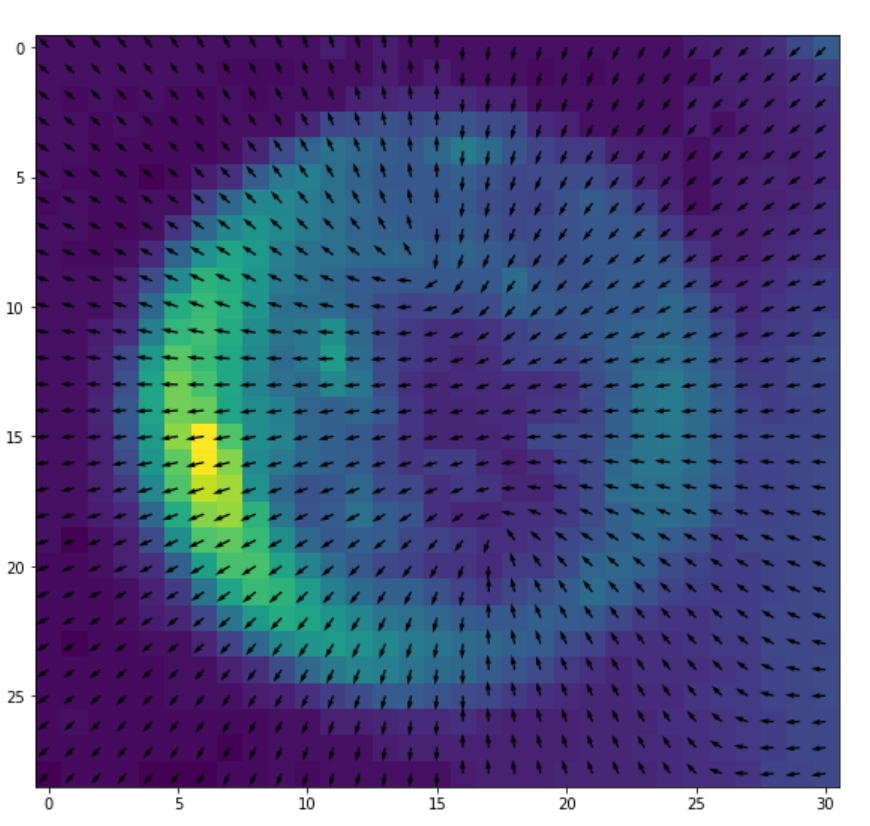
\includegraphics[scale=0.4]{images/structure_tensor_demo.png}
			\caption{Orientation angle using sobel filters for derivation and a Gaussian mask with $\sigma =1$ for smoothing.}
			\label{fig:struct_tensor_demo}
		\end{figure}
		
	
	\section{Machine Learning}
	\label{machine_learning}
	
	\section{The object detection problem}
	\label{the_object_detection_problem}
		\subsection{Evaluation Criteria}
